\documentclass[../thesis.tex]{subfiles}

\begin{document}

\chapter{Miscellaneous notes}
\label{chap:misc}

\section{Uncorrelated detection efficiency uncertainty}
\label{sec:miscDetEff}

In order to calculate proper errors on the oscillation parameters (particularly $\SinSq$), it is necessary to account for possible AD-to-AD variations in the IBD detection efficiency, as any such variations could potentially bias the measured rate deficit at the far site. As with the other systematics, this one is treated by the fitter's toy MC (\autoref{sec:toymc}): For each random set of toy prompt spectra, a random value is generated for each AD's efficiency, and its prompt spectrum is scaled accordingly. The covariance matrix generated from these prompt spectra then encodes the effects of the relative efficiency uncertainty. Here we briefly describe the determination of this uncertainty and its implementation in the toy MC.

The detection efficiency can be decomposed into various components, as detailed in \autoref{tab:detEff}. With the exception of the (dominant) first two rows (the delayed energy cut efficiency and the Gd capture fraction), the measurements of these components (and their AD-to-AD uncertainties) have remained unchanged since they were first described in \cite{SideBySide} and compiled in \cite{PhysRevLett.108.171803}.

Meanwhile, the first two rows of \autoref{tab:detEff} were updated in 2016 by Lebanowski in \cite{loganDetEff}, taking advantage of the increase in statistics since 2012. For the delayed energy cut, the uncorrelated efficiency uncertainty was evaluated by loosening the delayed cut to 3.6~MeV and comparing, between ADs, the percentage of delayed energies lying in the [6, 12]~MeV region. And for the nGd capture fraction, the prompt-delayed time difference for each AD was fit to an exponential in order to determine each AD's average capture time, which in turn gave the capture fraction. The spread of these capture fractions then gave the uncorrelated uncertainty.

\begin{table}[ht]
  \begin{tabular}{lc}
    \toprule
    Efficiency & Uncorrelated unc. (\%) \\
    \midrule
    Delayed energy & 0.075 \\
    Gd capture fraction & 0.1 \\
    Target protons & 0.03 \\
    Flasher cut & 0.01 \\
    Multiplicity cut & 0.01 \\
    Spill-in & 0.02 \\
    Capture time & 0.01 \\
    Prompt energy & 0.01 \\
    \midrule
    Total & 0.132 \\
    \bottomrule
  \end{tabular}
  \caption{Uncorrelated detection efficiency uncertainties \cite{loganDetEff}. Uncertainties were added in quadrature to obtain the total.}
  \label{tab:detEff}
\end{table}

An additional complication arises due to the correlation between the energy scale and the detection efficiency (via the delayed energy cut efficiency). When, in the toy MC, the energy scale is fluctuated, the detection efficiency must reflect this fluctuation, in addition to \emph{independent} fluctuations of the fraction of the efficiency that is \emph{not} correlated with the energy scale. The task is then to decompose the efficiency uncertainty into two parts, one correlated and one uncorrelated with the energy scale.

Nakajima carried out this decomposition in \cite{P15A_inputs}. His reasoning was as follows. First, the total efficiency uncertainty $\sigma_{\mathrm{tot}}$ (0.132\%) can be broken down into two parts: The 0.075\% uncertainty due to the delayed energy cut (which we denote $\sigma_{E_d}$), and the remainder ($\sigma_{\mathrm{other}}$):
\begin{equation}
  \sigma_{\mathrm{tot}} = 0.132\% = \sqrt{\sigma^2_{E_d} + \sigma^2_{\mathrm{other}}},
\end{equation}
where (\autoref{tab:detEff})
\begin{equation}
  \begin{aligned}
    \sigma_{E_d} &= 0.075\%. \\
    % \sigma_{\mathrm{other}} &= \sqrt{\sigma^2_{\mathrm{tot}} - \sigma^2_{E_d}} = 0.109\%
  \end{aligned}
\end{equation}
In turn, $\sigma_{E_d}$ is \emph{partially} correlated to the energy scale.
% We therefore break it down into two components:
% \begin{equation}
%   \sigma_{E_d} = \sqrt{\sigma^2_{E_d,\mathrm{corr}} + \sigma^2_{E_d,\mathrm{uncorr}}}.
% \end{equation}
According to \cite{loganDetEff}, 91.4\% of the AD-to-AD variance in the delayed energy cut efficiency is due to variance of the energy scale (\autoref{tab:delayedEffVariance}). Thus,
\begin{equation}
  \begin{aligned}
    \sigma_{\mathrm{corr}} &= \sqrt{0.914 \times \sigma^2_{E_d}} = 0.072\%. \\
    % \sigma_{E_d,\mathrm{uncorr}} &= \sqrt{(1 - 0.914) \times \sigma^2_{E_d}} = 0.022\%
  \end{aligned}
\end{equation}
We can then subtract (in quadrature) $\sigma_{\mathrm{corr}}$ from $\sigma_{\mathrm{tot}}$ to obtain the part of the detection efficiency uncertainty that is uncorrelated with the energy scale:
\begin{equation}
  \sigma_{\mathrm{uncorr}} = \sqrt{\sigma^2_{\mathrm{tot}} - \sigma^2_{\mathrm{\mathrm{corr}}}} = 0.11\%.
\end{equation}
In summary,
\begin{equation}
  \begin{aligned}
    \sigma_{\mathrm{tot}} &= \sqrt{\sigma^2_{\mathrm{corr}} + \sigma^2_{\mathrm{uncorr}}} \\
    &= \sqrt{(0.072\%)^2 + (0.11\%)^2}.
  \end{aligned}
\end{equation}

\begin{table}[ht]
  \begin{tabular}{lc}
    \toprule
    Component & Fraction (\%) \\
    \midrule
    Energy scale & 91.4 \\
    OAV thickness & 7.8 \\
    Nonuniformity & 0.8 \\
    \bottomrule
  \end{tabular}
  \caption{Decomposition of the variance of the delayed energy cut efficiency \cite{loganDetEff}.}
  \label{tab:delayedEffVariance}
\end{table}

As described in \cite[Sec.\@ III B 5 b]{An_2017}, the AD-to-AD variation of the energy scale, $\delta_E$, is $\sim$0.20\%. It is then assumed that this 0.20\% variation leads to the observed 0.072\% energy-scale-correlated detection efficiency variation $\delta_{\epsilon_d}$:
\begin{equation}
  0.072\% = \frac{\delta_{\epsilon_d}}{\delta_E} \times 0.20\%,
\end{equation}
or
\begin{equation}
  \frac{\delta_{\epsilon_d}}{\delta_E} = \frac{0.072}{0.20} = 0.36.
\end{equation}
Therefore,
\begin{equation}
  \delta_{\epsilon_d} = 0.36 \times \delta_E.
\end{equation}

In the toy MC, after a fractional energy scale fluctuation $\delta_E$ is generated via $\Gaus(0, 0.0020)$, the nominal\footnote{And arbitrary, since we are performing a relative measurement.} detection efficiency is first multiplied by $1 + 0.36 \times \delta_E$. The result is then multipled by an additional factor of $1 + \Gaus(0, 0.0011)$ to account for the detection efficiency variance that is uncorrelated with the energy scale. That is,
\begin{equation}
  \epsilon_d = \epsilon_{d,\mathrm{nom}} \cdot (1 + 0.36 \times \Gaus(0, 0.0020)) \cdot (1 + \Gaus(0, 0.0011)),
\end{equation}
where the first Gaussian random variable is the same one used in fluctuating the energy scale. This gives the final detection efficiency used by the toy MC. The prompt spectrum is uniformly scaled by this factor in generating the toy sample.

\section{Energy nonlinearity model}
\label{sec:reconEnergyNLDetails}

The AD's response on the type of particle in question. By construction, AdSimple's $\Erec$ will report the correct deposited energy for the $\sim$8~MeV gamma-ray peak produced by nGd capture. However, due to the various sources of nonlinearity (from quenching, Cherenkov emission, and the electronics, as summarized in \autoref{sec:reconEnergyNL} and detailed below), $\Erec$ will report a different value for a \emph{positron} that deposits 8~MeV. As described below, this effect must be considered when constructing the conversion between $E_{\mathrm{rec}}$ and $E_{\mathrm{dep}}$ for positrons.\footnote{Given that, for the purpose of oscillation physics, the IBD positron spectrum is the only one whose shape carries any significance, there is no need in this analysis to apply separate corrections for purported gamma ray, electron, or alpha particle events. Indeed, the delayed (i.e. nGd gamma ray) spectrum does not undergo any nonlinearity correction here.}) All in all, the ratio of $E_{\mathrm{rec}}$ to $E_{\mathrm{dep}} $varies by some 10\% across the range of energies used in the analysis (0.7--12~MeV). If this nonlinearity is not corrected for,\footnote{The nonlinearity correction is not actually performed during reconstruction. Instead, the correction is applied by the fitter (\autoref{chap:fitting}), which takes AdSimple's $\Erec$ and converts it into $\Enu$. However, as this is merely an implementation detail, we discuss the conversion in this chapter, along with the other preceding steps of the energy reconstruction.} then the resulting distortion in the IBD positron spectrum will potentially bias the extraction of $\Dmsqee$.

The nonlinearity correction thus converts $E_{\mathrm{rec}}$ into $E_{\mathrm{dep}},$ which can then be trivially converted to the true neutrino energy, $\Enu$, using \autoref{eq:enuToEdep}:
\begin{equation}
  \Enu \simeq \Edep + \SI{0.80}{MeV} 
\end{equation}.
In what follows, the phrase ``positron energy'' refers to $E_{\mathrm{dep}}$, which can be trivially related to the kinetic energy $E_{\mathrm{kin}}$ and the relativistic energy $E_{\mathrm{rel}}$ via
\begin{equation}
  \Edep = E_{\mathrm{kin}} + 2m_e = E_{\mathrm{rel}} + m_e.
\end{equation}

The scintillator (quenching + Cherenkov)  and electronics nonlinearities are both on the scale of 10\%, and work in opposite directions: The scintillator response is suppressed for low-energy events, while the electronics show a reduced response for high-energy events. Nevertheless, they do not cancel each other very effectively, so each must be treated separately and carefully. We begin with the scintillator. In terms of physical processes, the scintillator nonlinearity determines $\Evis$ from $\Edep$, and then the electronics nonlinearity determines $\Erec$ from $\Evis$. In analysis, this logic is reversed in order to determine $\Edep$ given $\Erec$\footnote{Recall that any effects from geometric nonuniformity have already been removed in the computation of $\Erec$.}.

In detailing the nonlinearity correction, we begin by discussing the AD's response to electrons, rather than positrons. For organic scintillators such as the Daya Bay LS, quenching is quantitatively well described by \emph{Birks' law} \cite{Birks_1951},
\begin{equation}
  \frac{dQ}{dx} \propto \frac{\frac{dE}{dx}}{1 + k_B \frac{dE}{dx}}
  \label{eq:reconBirks}
\end{equation}
where $Q$ is the amount of emitted light, $dE/dx$ is the linear density of \emph{ionization} energy deposition, and the scintillator-specific value $k_B$ is known as Birks' constant.

If the $dE/dx$ profile is known across a particle's range, then it can be used to integrate \eqref{eq:reconBirks}. Such a ``semi-empircal'' analytic approach was used to compute the shape of the quenching curve for electrons in the Daya Bay LS \cite{NonlinearityPaper}. This relationship was encoded in a function denoted $f_q(\Edepelec, k_B)$, where $k_B$ remained to be determined from data:
\begin{equation}
  f_q(\Edepelec,k_B) = \int_0^{\Edepelec} \frac{\frac{dE}{dx}}{1 + k_B \frac{dE}{dx}}.
  \label{eq:reconBirksInt}
\end{equation}
Plots of $f_q$ for different values of $k_B$ are shown in \autoref{fig:reconBirksInt}.

\begin{figure}[h]
  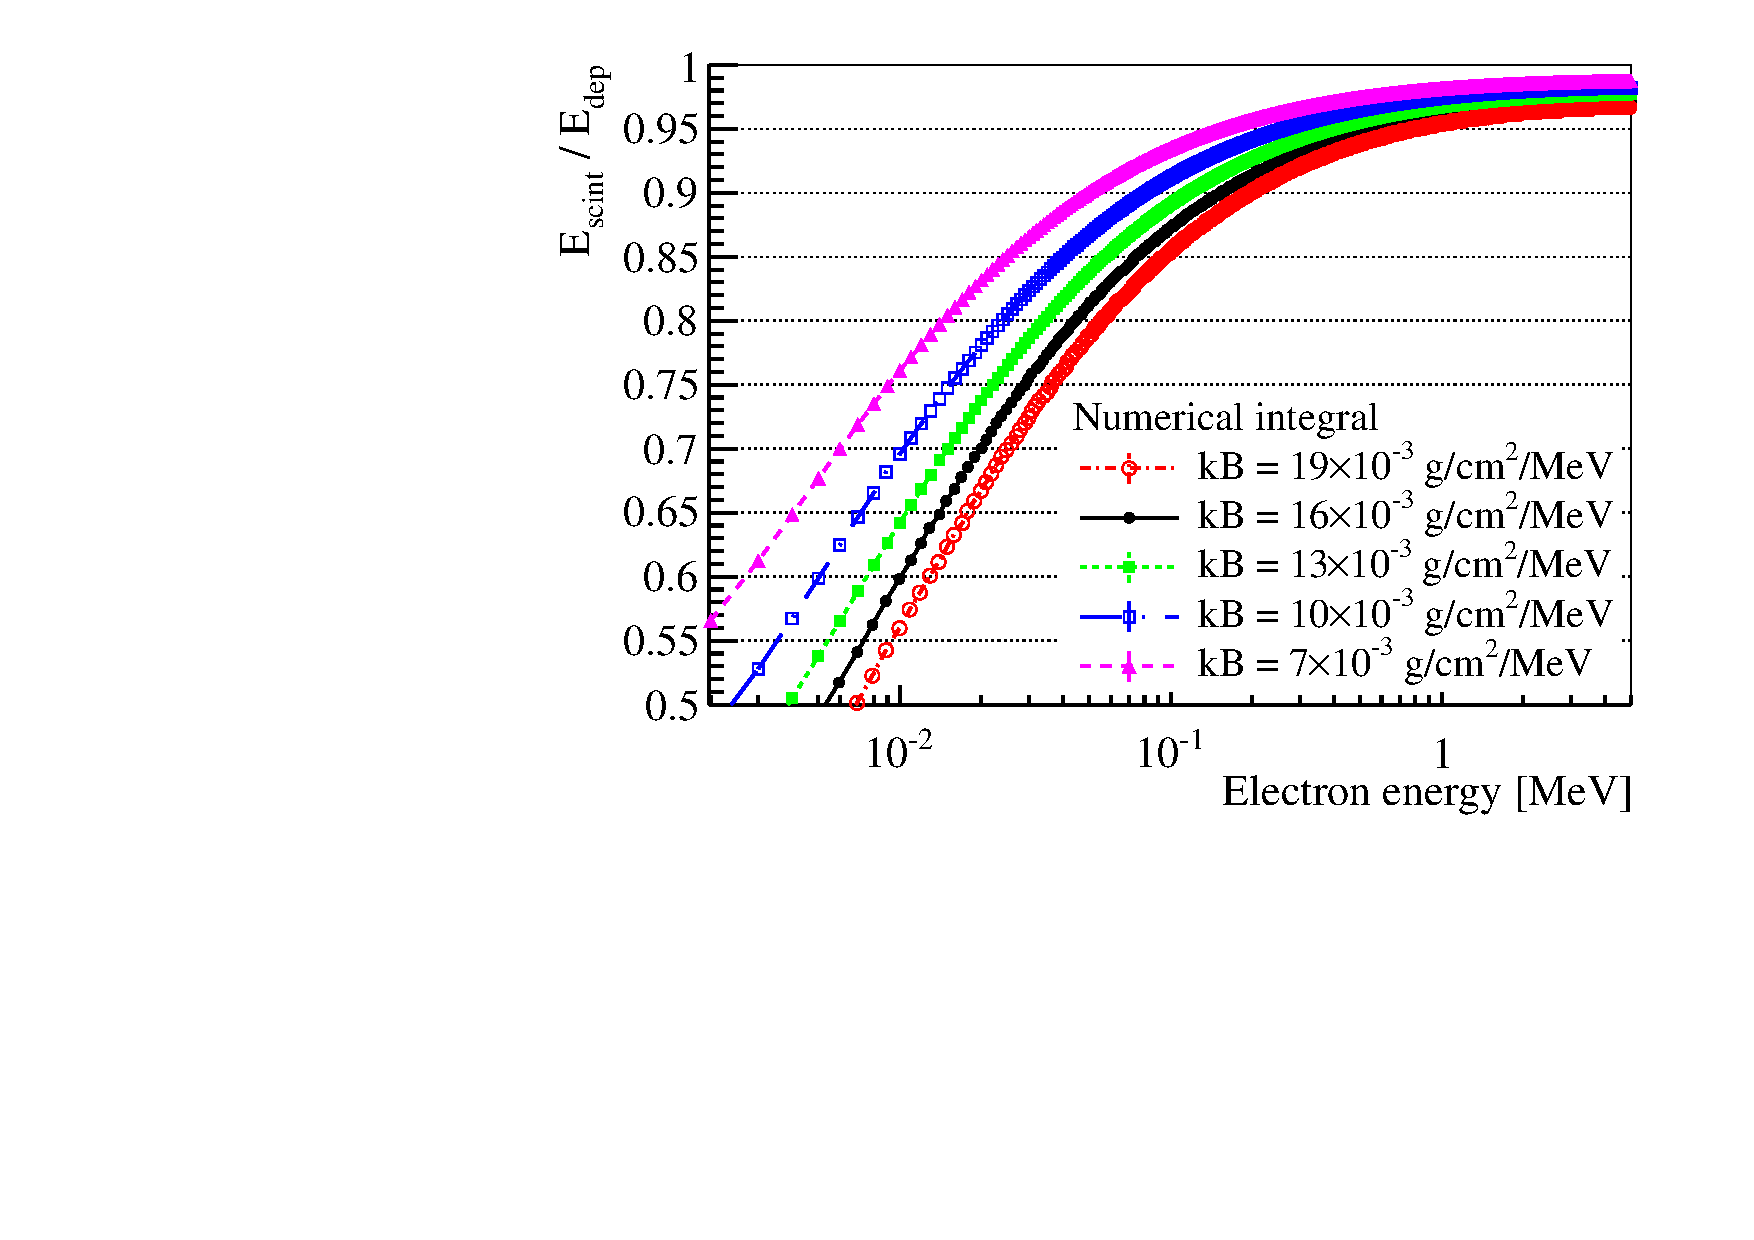
\includegraphics[scale=0.5]{Reconstruction/s04_Quench_kb.pdf}
  \caption{Dependence of the scintillation energy on the deposited energy of electrons, for various values of Birks' constant $k_B$. From \cite{NonlinearityPaper}.}
  \label{fig:reconBirksInt}
\end{figure}

Although Cherenkov emission is the sole source of light in the Daya Bay water pools, it plays a subpercent role in the ADs. The energy dependence of Cherenkov emission was determined from Geant4 simulations (and independently confirmed by an analytic calculation), giving the tabulated function $f_c(\Edepelec)$ (\autoref{fig:cerenkovShape}), which was arbitrarily assigned a ($k_B$-dependent) normalization such that $f_c(\SI{1}{MeV}) = f_q(\SI{1}{MeV}, k_B)$. 

\begin{figure}[h]
  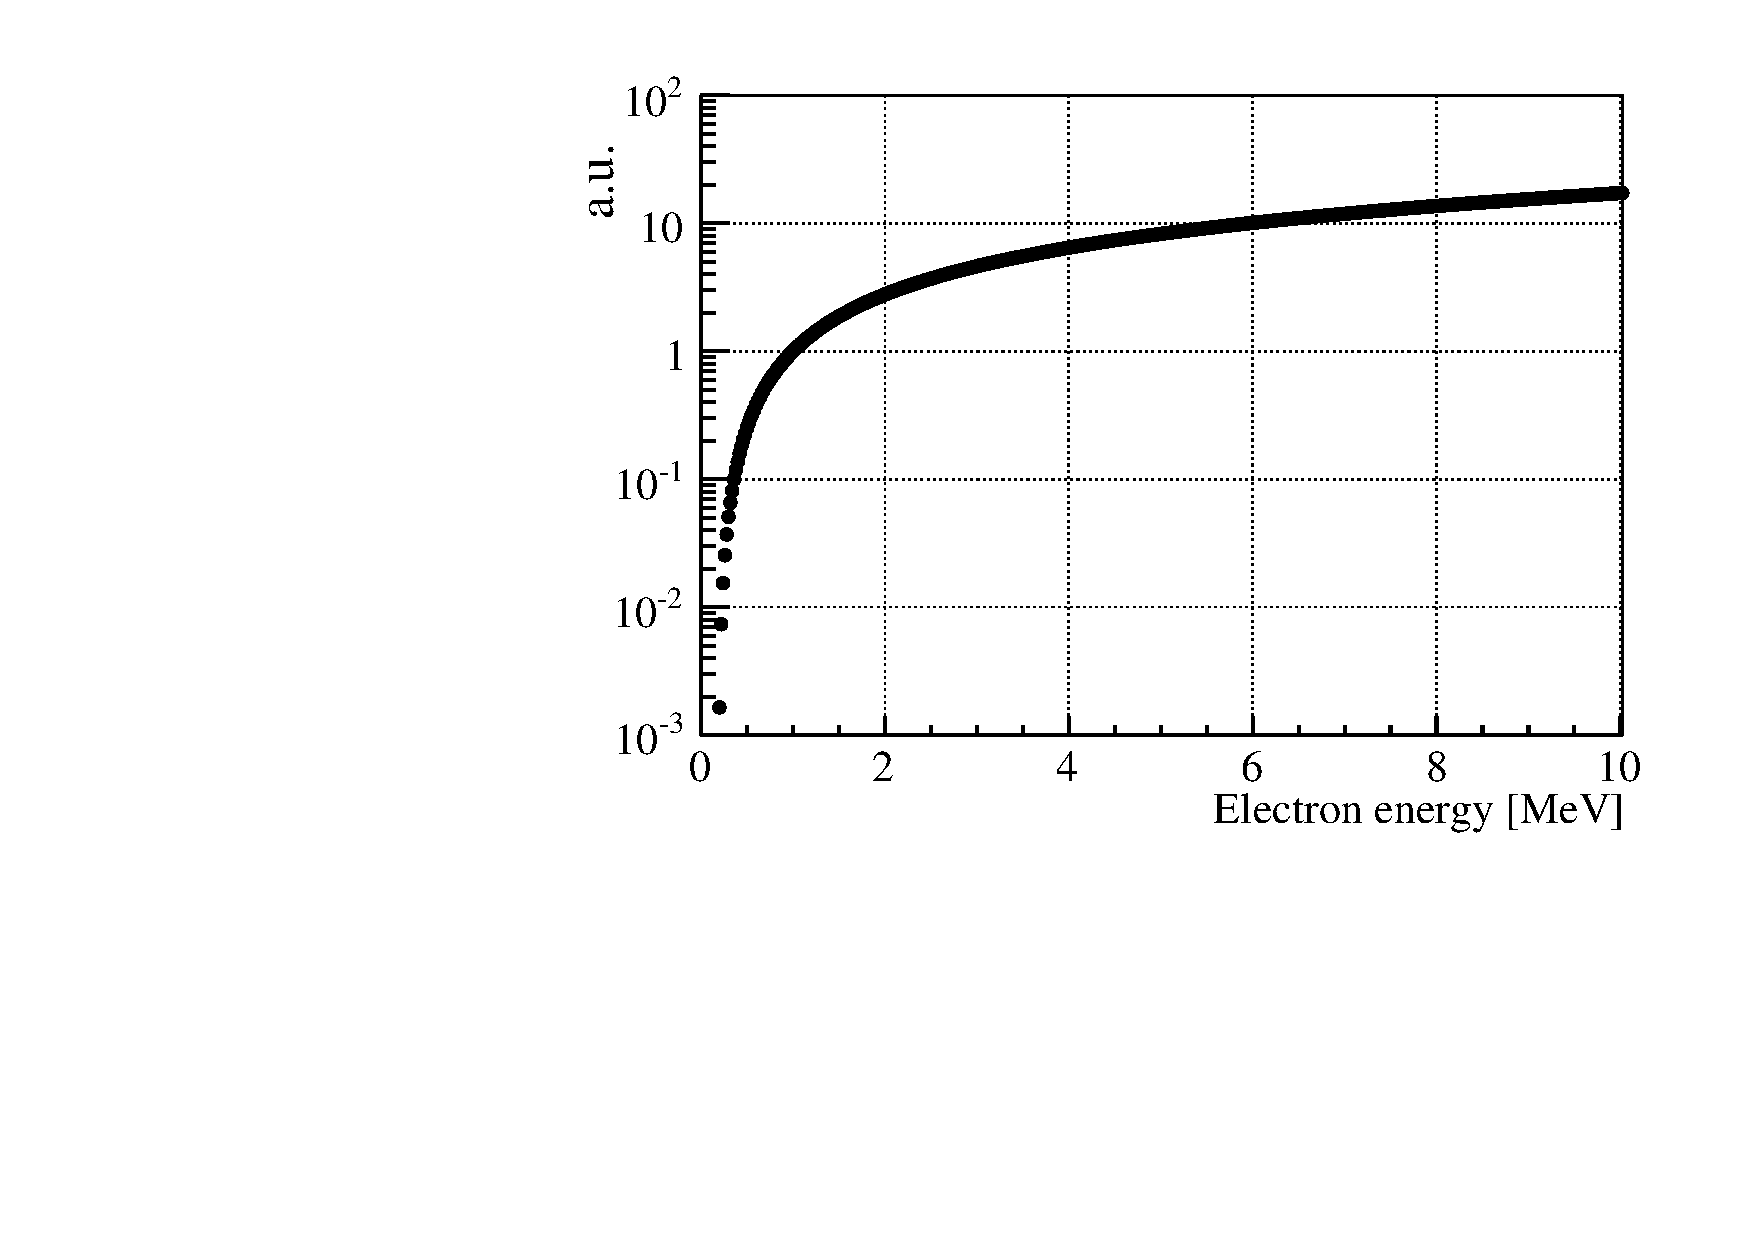
\includegraphics[scale=0.5]{Reconstruction/s04_CerenkonContribution.pdf}
  \caption{Energy dependence of the Cherenkov contribution to light emission by electrons in the LS (here, arbitrarily normalized at 1~MeV), from \cite{NonlinearityPaper}. The actual normalization of this function was determined by a fit to measurements of the nonlinearity, as described in \cite{NonlinearityPaper}.}
  \label{fig:cerenkovShape}
\end{figure}

Altogether, the combined effects on electrons of quenching and Cherenkov emission are therfore described by the relation
\begin{equation}
  \label{eq:reconScintNonlin}
  \frac{E_{\mathrm{vis},e^-}}{\Edepelec} = \beta_{\mathrm{vis}}[f_q(\Edepelec, k_B) + k_c f_c(\Edepelec)],
\end{equation}
where $f_q$ is given by \autoref{eq:reconBirksInt}, and $f_c$ (which, being tabulated from simulation data, cannot be expressed as an equation) is, again, shown in \autoref{fig:cerenkovShape}. Here, we have introduced the constant $k_c$, which describes the ratio of the amount of Cherenkov emission to scintillation. $\beta_{\mathrm{vis}}$ is an arbitrary normalization. The parameters $k_B$ and $k_c$ are determined from data, as will be described shortly.

Thus far we have only discussed the response of the scintillator to electrons. The end goal, however, is to characterize the response to \emph{positrons,} since that is what will allow the measurement of the antineutrino spectrum. Before the positron annihilates, it effectively ionizes the medium in the same manner as an electron would. Following ionization, we measure the response of the scintillator to two 511~keV gamma rays. Accordingly,
\begin{equation}
  \label{eq:reconScintPositron}
  E_{\mathrm{vis},e^+}(E_{\mathrm{kin}}) = E_{\mathrm{vis},e^-}(E_{\mathrm{kin}}) + 2 \times E_{\mathrm{vis},\gamma}(\SI{0.511}{MeV}).
\end{equation}

Gamma rays, in turn, do not themselves ionize, but they do produce and scatter electrons and positrons. The total response to gamma rays is, accordingly, rather complex, given the need to account for annihilation and pair production \emph{ad nauseam}. As such, Geant4 simulation were used to determine the response of the scintillator to gamma rays, as a function of $k_B$ and $k_c$. The (ionization) energy deposited by each simulated electron and positron (\autoref{fig:reconGammaElectrons}) was converted into visible energy according to \eqref{eq:reconScintNonlin}, and the sum gave the visible energy from each gamma ray. With the response to gamma rays thus determined, it could be plugged into \eqref{eq:reconScintPositron} to give the response to positrons.

\begin{figure}[h]
  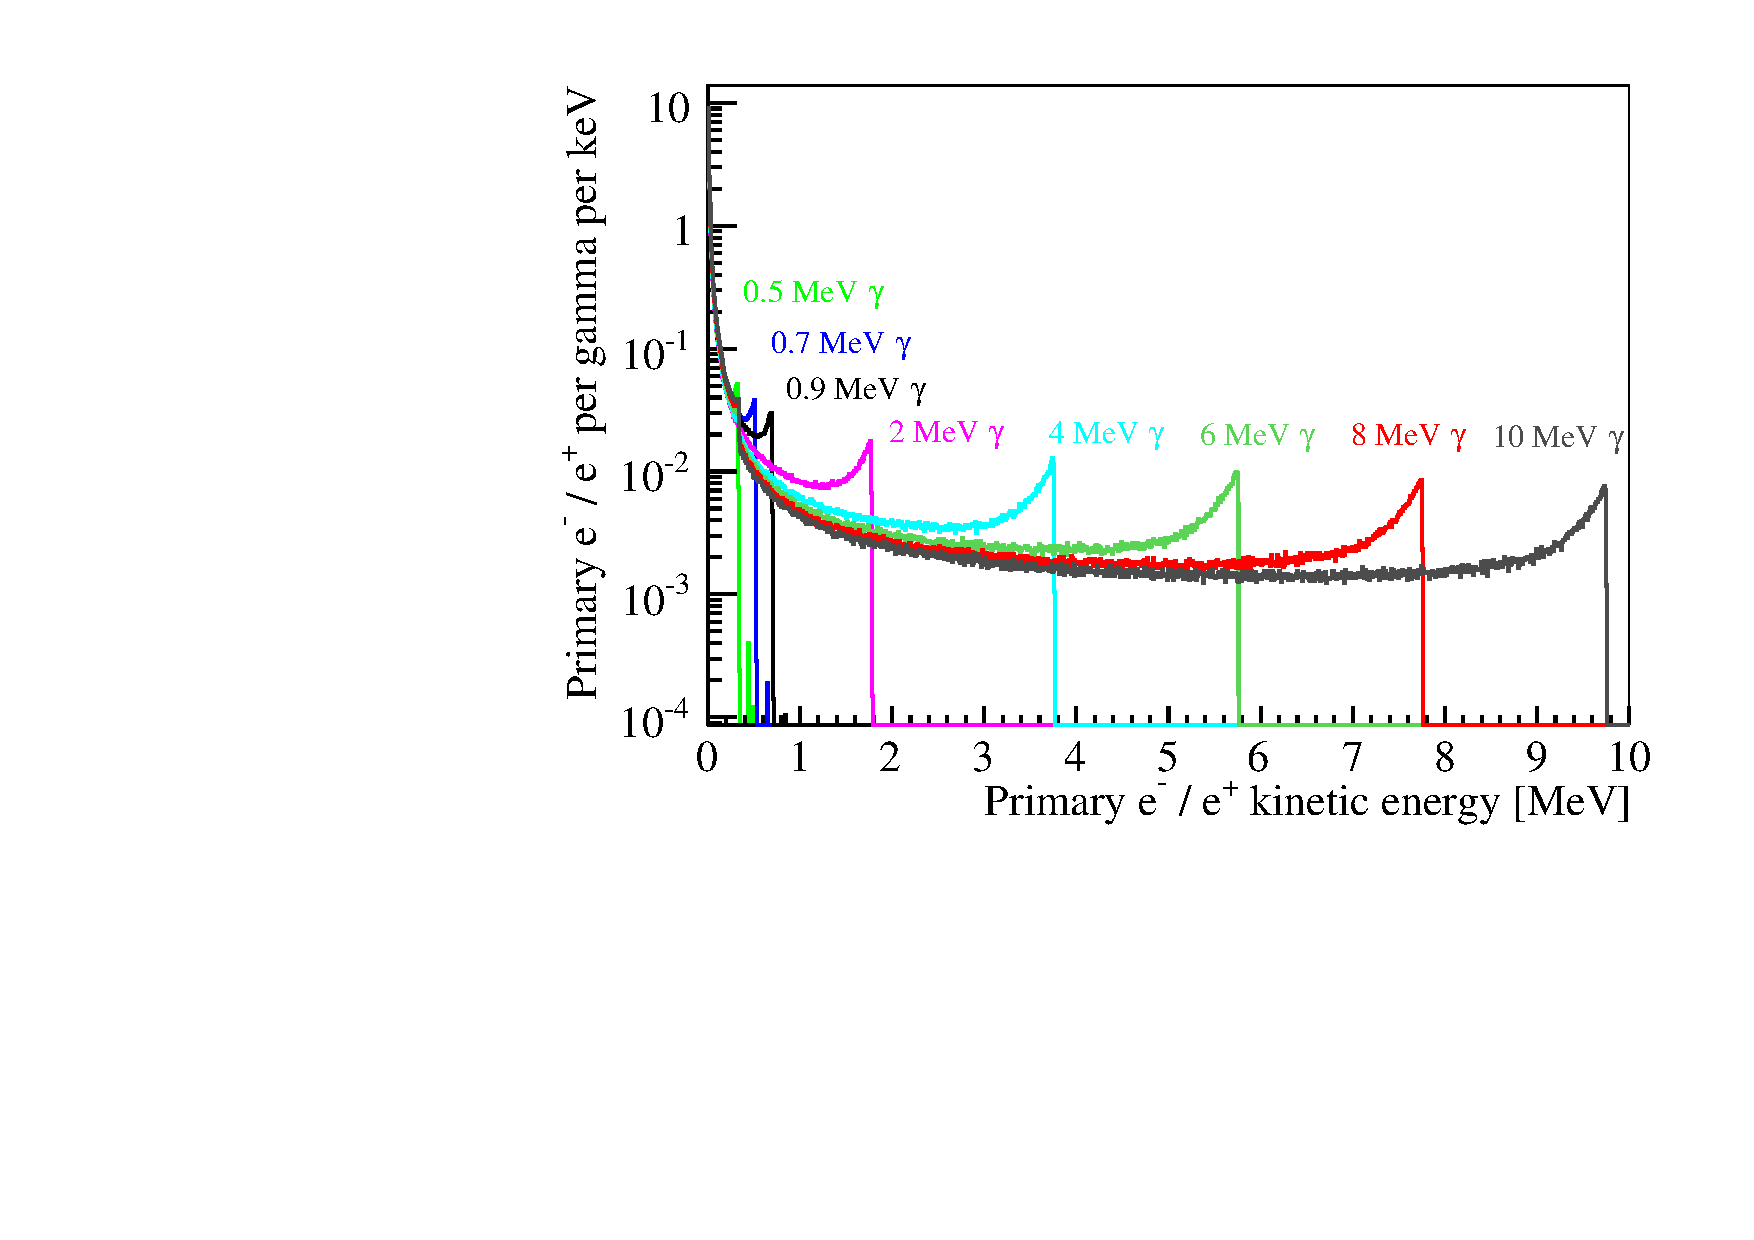
\includegraphics[scale=0.5]{Reconstruction/s04_Gamma_electron.pdf}
  \caption{Distribution of kinetic energies of electrons produced by gamma rays of a variety of initial energies. From \cite{NonlinearityPaper}.}
  \label{fig:reconGammaElectrons}
\end{figure}

In addition to the nonlinear light \emph{emission} of the scintillator, there is also nonlinear light \emph{measurement} caused by the design of the electronics. As was described in \autoref{sec:reconHitSelection}, the charge (i.e. light) in each channel is determined by taking the \emph{first} hit within the nominal time window. And as was described in \autoref{sec:calibHitCharge}, the first hit will tend to accurately measure the light observed by the PMT, \emph{provided that all of the photons arrived within 100~ns of each other.} However, some 5\% of the light is from the slow component, and will therefore arrive too late to be captured by the hit that corresponds to the fast/medium light. Thus, high-energy events, in which every channel ``sees'' some fast/medium light, will fail to record any of the slow light. Conversely, in a lower-energy event, some of the slow light \emph{will} be recorded, since there is not enough fast/medium light to hit every channel. This means that the electronics response is slightly suppressed for high-energy events and slightly enhanced for low-energy ones.

Based on a combination of measurements and simulations, this behavior was found to be adequately described by the relation
\begin{equation}
  \frac{\Erec}{\Evis} = \beta_{\mathrm{rec}}\left[ 1 + \alpha \left( - \frac{\Evis}{\tau} \right) \right],
  \label{eq:reconScintElec}
\end{equation}
where $\alpha$ and $\tau$ are, like $k_B$ and $k_c$, constrained by measurements, and $\beta_{\mathrm{rec}}$ is, like $\beta_{\mathrm{vis}}$, merely an arbitrary normalization. The product $\beta_{\mathrm{vis}}\beta_{\mathrm{rec}}$, by convention, is chosen to ensure that $\Erec = \Edep$ for 8~MeV electrons.

In order to determine the four parameters $k_B$, $k_c$, $\alpha$, and $\tau$ of the nonlinearity model, a fit was performed to a dataset consisting of the peaks from twelve gamma rays (from deployed sources and natural radioactivity) as well as the electron spectrum from decays of cosmogenic $^{12}$B \cite{NonlinearityPaper}, as shown in \Autoref{fig:reconGammaLines,fig:reconB12}. The measured values of $\Erec$ were compared to those predicted by simulation (for a given set of the parameters), and the best-fit parameters were determined as those that minimized the $\chi^2$ between measurement and prediction. As no significant differences in nonlinearity were observed between ADs, a single nonlinearity model is used for all eight. The best-fit parameters were found to be $k_B = 15 \times 10^{-3}\;\mathrm{cm\, MeV^{-1}}$, $k_c = 0.5\%$, $\alpha = 0.078$, and $\tau = \SI{2.55}{MeV}$. However, these values depend on the assumed shapes $f_q$ and $f_c$, which in turn depend on the configuration of Geant4. Accordingly, our analysis does not make direct use of these four parameters; instead we use the digitized nonlinearity curve published in \cite{NonlinearityPaper}, as shown in \autoref{fig:reconPositronNominal}, which includes a 68\% uncertainty band (derived from the $\chi^2$ fit), corresponding to a precision of about 1\%.

\begin{figure}[h]
  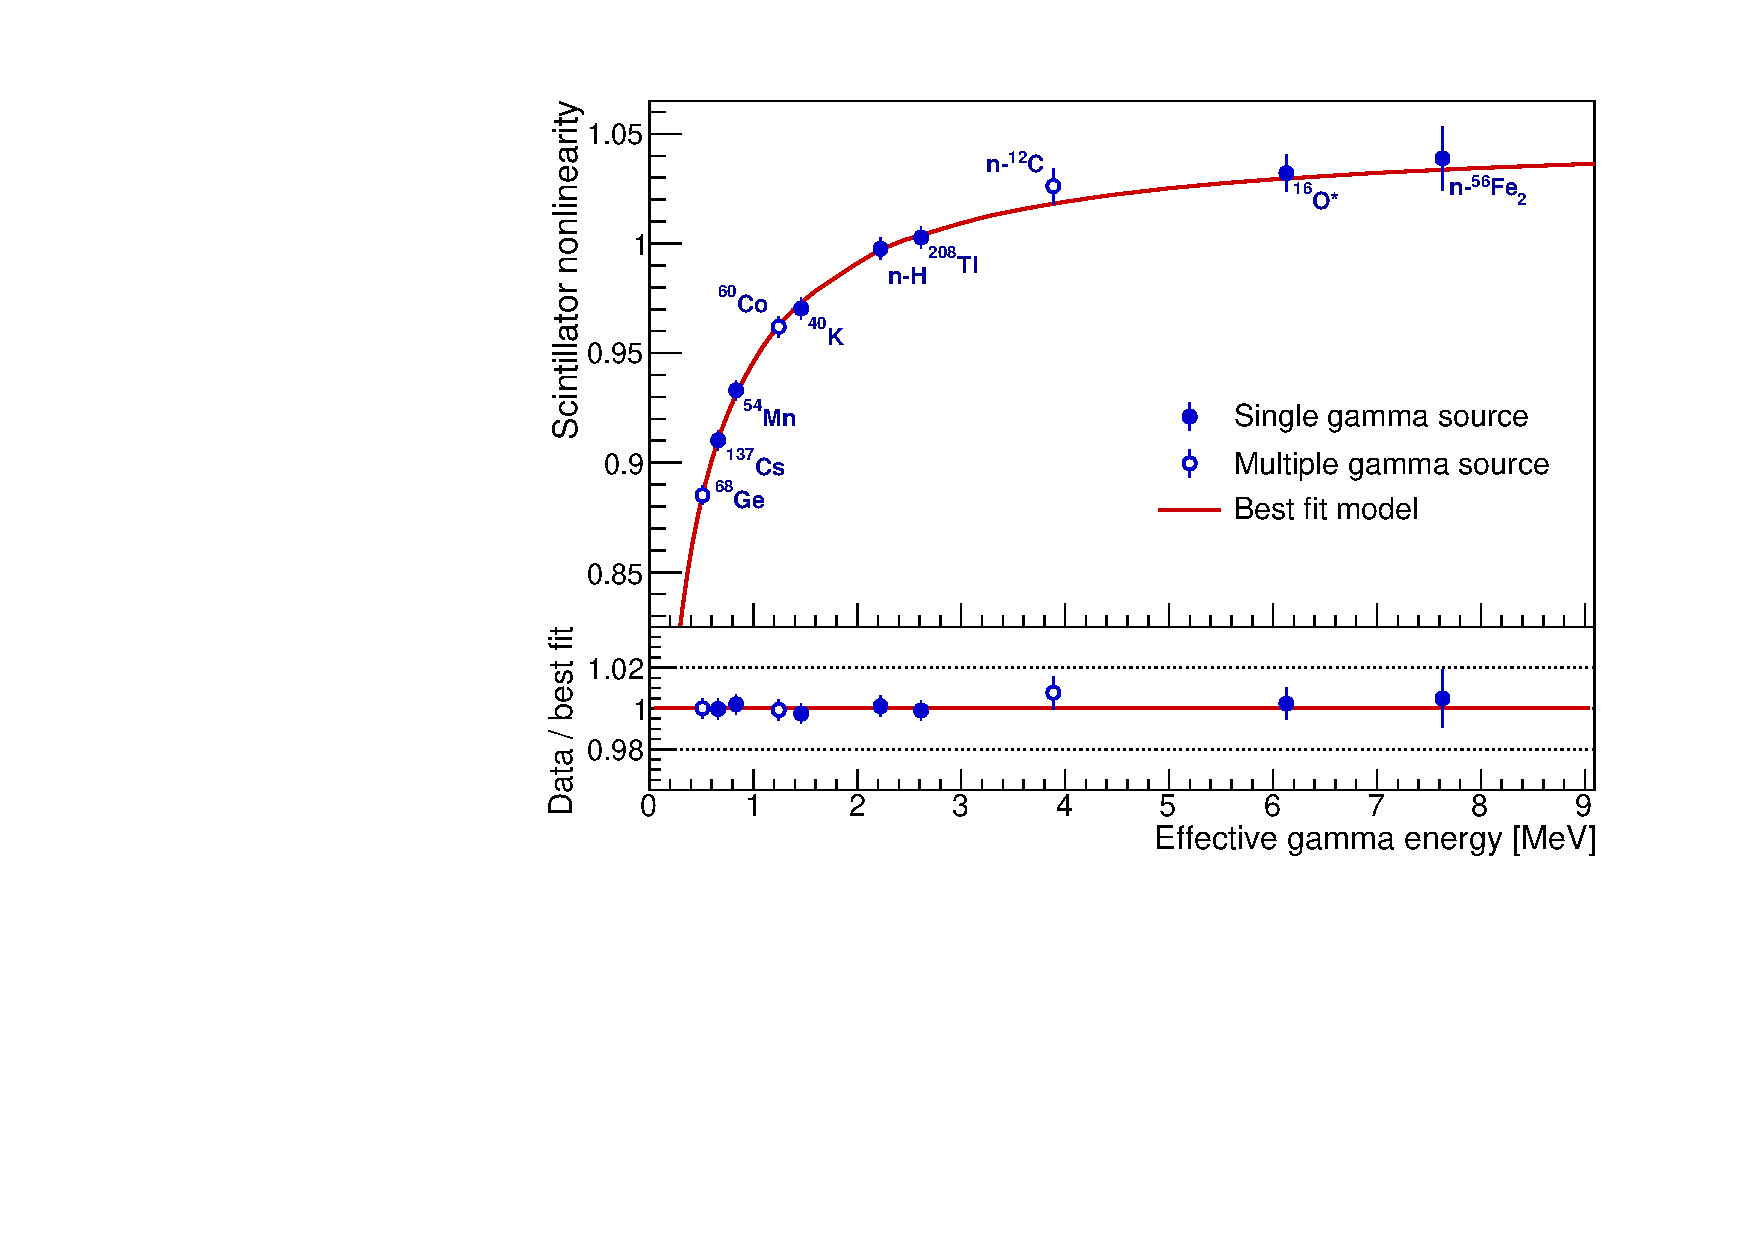
\includegraphics[scale=0.5]{Reconstruction/s06_LSNL_bestfit.pdf}
  \caption{Measured LS nonlinearity for various energies of gamma-rays. From \cite{NonlinearityPaper}.}
  \label{fig:reconGammaLines}
\end{figure}

\begin{figure}[h]
  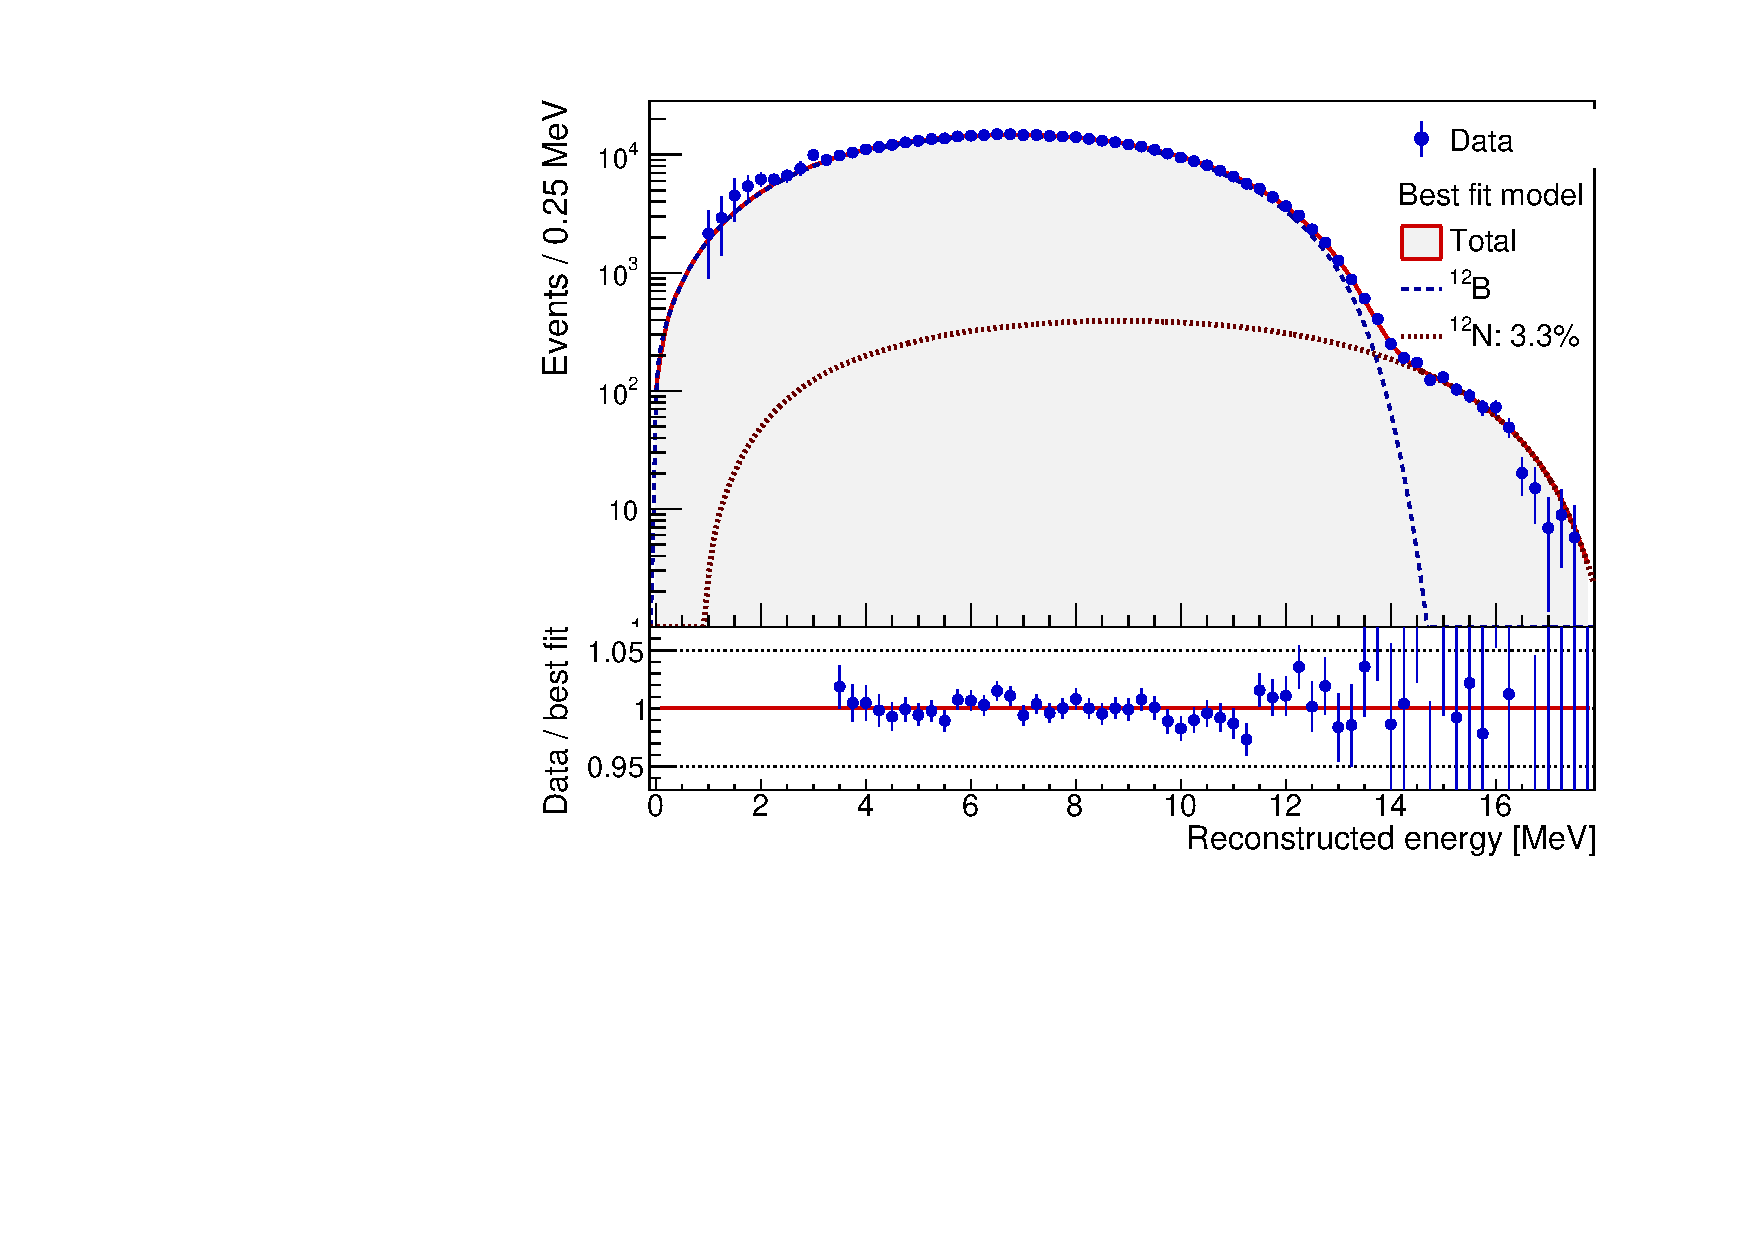
\includegraphics[scale=0.5]{Reconstruction/s06_B12_bestfit.pdf}
  \caption{The reconstructed energy spectrum from $^{12}$B (with a minor contribution from $^{12}$N). Also shown is the prediction obtained from the best-fit nonlinearity model (equations \autoref{eq:reconScintNonlin} $\times$ \autoref{eq:reconScintElec}). From \cite{NonlinearityPaper}.}
  \label{fig:reconB12}
\end{figure}

\begin{figure}[h]
  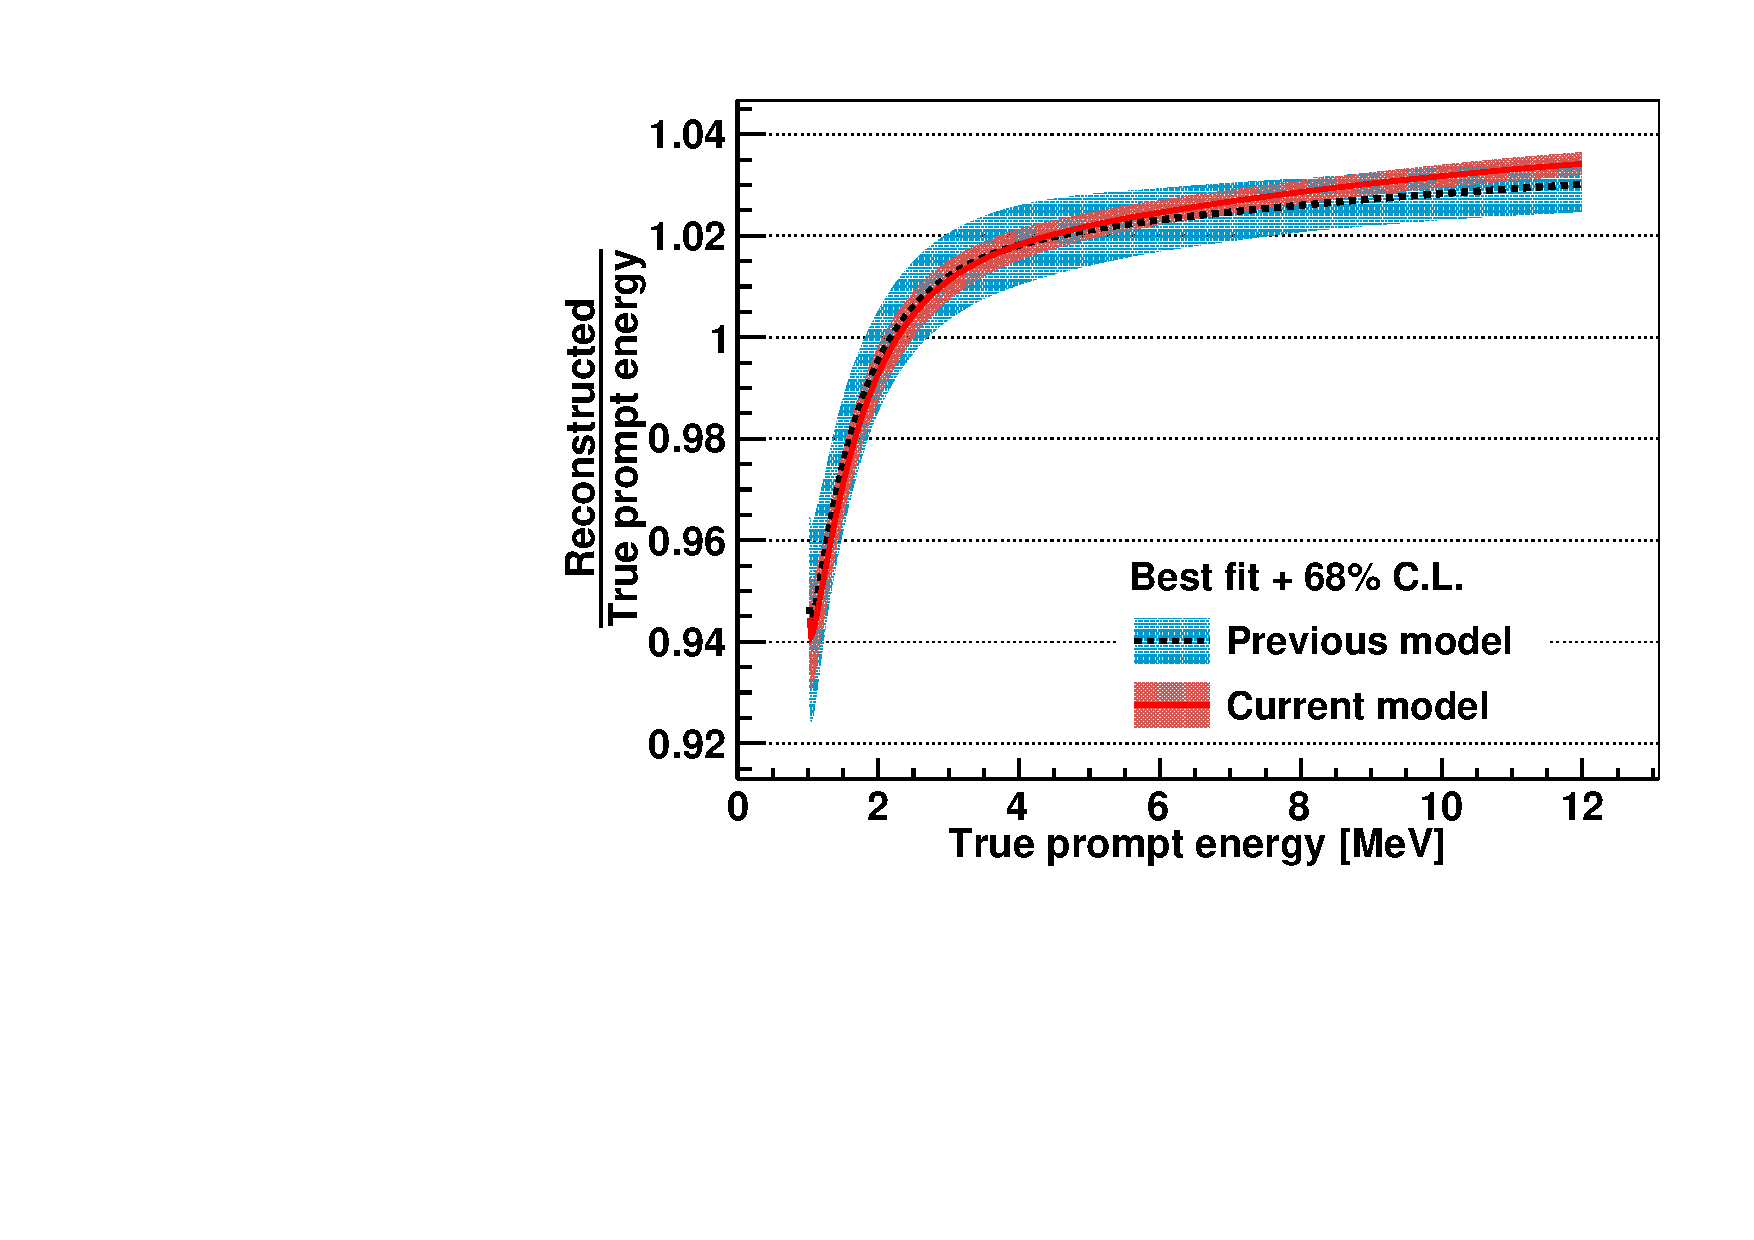
\includegraphics[scale=0.5]{Reconstruction/s06_PositronNominal.pdf}
  \caption{Best-fit nonlinearity model for positrons. From \cite{NonlinearityPaper}.}
  \label{fig:reconPositronNominal}
\end{figure}

The scintillator nonlinearity was cross-checked using the 53-MeV Michel electron from muon decay as well as the $\beta+\gamma$ spectra from $^{212}$Bi, $^{214}$Bi, and $^{208}$Tl decays, while the electronics nonlinearity was validated using data from a fast ADC system that directly recorded the PMT waveforms in one AD \cite{HUANG201848}. Further validation involved verifying that the best-fit model remained stable under removal of any single calibration point. The results of these studies were consistent with the uncertainty band of the nonlinearity model.

\section{Vertex reconstruction}
\label{chap:vertexReconDetails}

The AdSimple vertex reconstruction proceeds in multiple stages \cite{adsimple1,adsimple2}, as shown in \autoref{fig:vtx_rec_flow}. First, an initial vertex is determined by taking a simple \emph{center of charge} (COC) using the coordinates of the PMTs. As this method suffers from significant biases (largely toward the center of the AD), a correction is then applied, based on interpolating a map of the mean bias (as a function of COC position) determined from a sample of Monte Carlo events, giving the \emph{Monte Carlo Corrected COC} (MCC-COC). However, even with the MC correction, this vertex still suffers from biases, particularly at large $z$ (\autoref{fig:reconMccCocWiggles}). In order to reduce such effects, and to also improve the resolution of the position reconstruction, a final vertex is computed by matching the distribution of PMT charges to a library of MC templates. We now discuss these steps in further detail. 

\begin{figure}[h]
  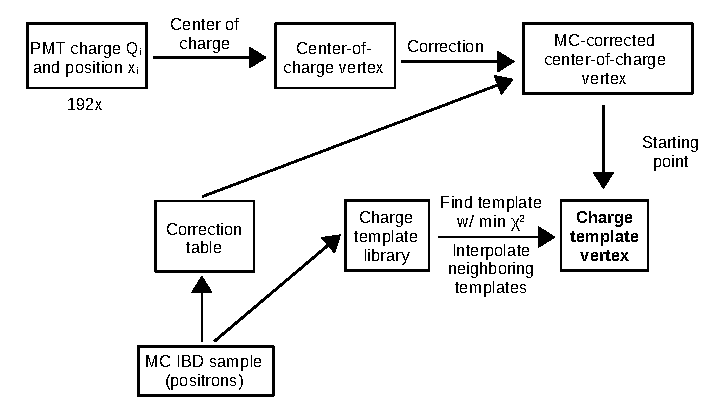
\includegraphics[scale=1.0]{Reconstruction/vtx_rec_flow.pdf}
  \caption{Flowchart of the steps involved in the AdSimple vertex reconstruction.}
  \label{fig:vtx_rec_flow}
\end{figure}


\begin{figure}[h]
  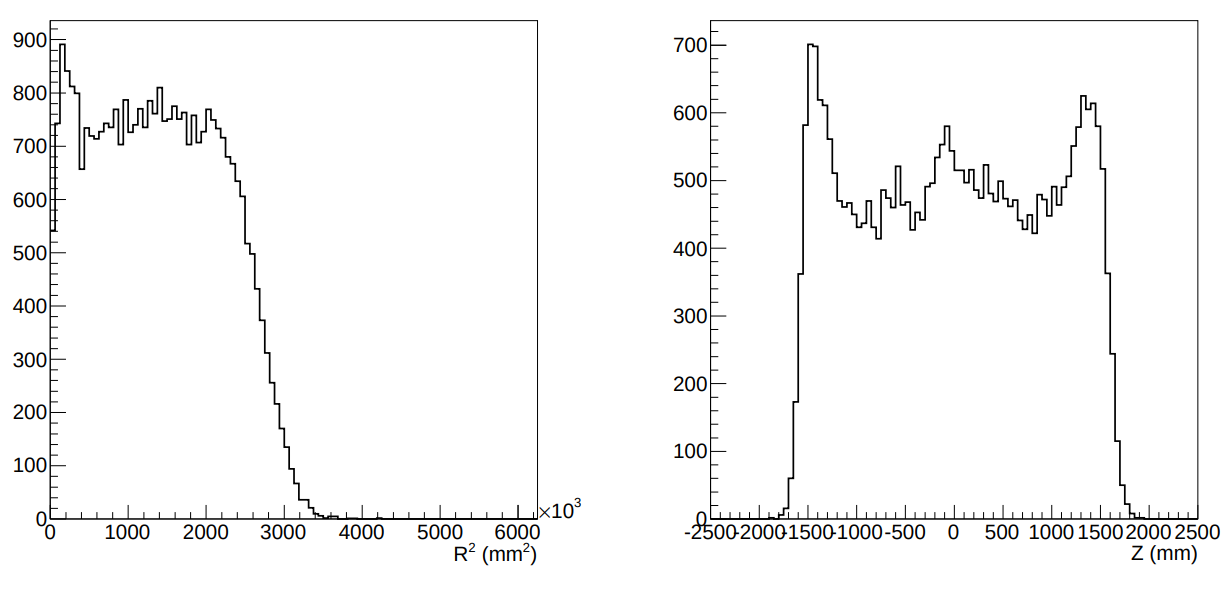
\includegraphics[scale=0.4]{Reconstruction/mcc_coc_wiggles_positron.png}
  \caption{Biases in the MCC-COC vertex distributions for positrons associated with IBD neutrons. The true distribution of events is uniform in the GdLS. From \cite{adsimple1}.}
  \label{fig:reconMccCocWiggles}
\end{figure}

The COC vertex is calculated trivially,
\begin{equation}
  x_{\mathrm{COC}} = \frac{\sum_{i}^{\mathrm{PMTs}} Q_i \vec{x_i}}{\sum_i^{\mathrm{PMTs}} Q_i},
\end{equation}
where $\vec{x_i}$ is the position of the $i$th PMT (in Cartesian coordinates, with the origin at the AD's center), and $Q_i$ is the corresponding observed charge in photoelectrons (without any correction for electronics nonlinearity). To this vertex, the correction from MC is applied next.

The MC sample consists of a large number of uniformly-distributed IBD events, generated using the ILL-Vogel flux model without oscillation (see \autoref{tab:mccCocMcSampleCoefs}). A cut is applied on the true interaction to eliminate events that occur outside the OAV. The positrons (i.e. prompt triggers) from these events are then used to generate a correction table.

\begin{table}[h]
  \begin{tabular}{lr}
    \toprule
    Isotope & Fraction \\
    \midrule
    $^{235}$U & 0.60 \\
    $^{238}$U & 0.05 \\
    $^{239}$Pu & 0.30 \\
    $^{241}$Pu & 0.05 \\
    \bottomrule
  \end{tabular}
  \caption{Nominal fission fractions used when employing the ILL-Vogel model to generate simulated IBD events for constructing the MC correction table for the MCC-COC.}
  \label{tab:mccCocMcSampleCoefs}
\end{table}

For each MC event, the COC vertex is calculated, and two corrections, a ``radial'' and a ``vertical'' one, are computed (using cylindrical coordinates, again with the origin at the AD's center):
\begin{equation}
  \Delta r = \frac{\vec{r}_{\mathrm{true}} \cdot \vec{r}_{\mathrm{COC}}}{\abs{\vec{r}_{\mathrm{COC}}} - r_{\mathrm{COC}}},
\end{equation}
\begin{equation}
  \Delta z = z_{\mathrm{true}} - z_{\mathrm{COC}},
\end{equation}
Events are divided into 20 bins for $\SI{0}{m} < r_{\mathrm{COC}} < \SI{2}{m}$ and 40 bins for $\SI{-2}{m} < z_{\mathrm{COC}} < \SI{2}{m}$. For each bin, the mean $\Delta z$ is computed, while the mean $\Delta r$ is computed over (and assigned to) all $z{_\mathrm{COC}}$ bins for a given $r_{\mathrm{COC}}$, since there is very little $z$ dependence on $\Delta r$. The $\Delta r$ and $\Delta z$ correction tables are ``pre-interpolated'' with a spline function\footnote{Unfortunately, it was not possible to find a record of the exact spline function used. Presumably, it was a quadratic or cubic function. In any case, since the MCC-COC is ultimately only used as a ``pre-fit'' starting point for the template-based reconstruction, its precise details are not extremely important.} to give a $\times$10-finer grid, which is then stored for use by AdSimple. During reconstruction, linear interpolation is applied to this fine-binned grid to look up the corrections for arbitary ($r_{\mathrm{COC}}$, $z_{\mathrm{COC}}$). Application of the correction is trivial: $r \mapsto r + \Delta r$ and $z \mapsto z + \Delta z$. This gives the MCC-COC vertex.

The final stage of the AdSimple vertex reconstruction relies on a library of 9,600 charge templates (i.e. distributions of charge across the PMTs), with each template corresponding to a voxel of the detector. These voxels (i.e. bins) are defined as the product of 20 bins in $\SI{0}{\square m} < r^2 < 2^2\;\mathrm{m}^2$, 20 bins in $\SI{-2}{m} < z < \SI{2}{m}$, and 24 bins in $0 < \phi < 2\pi$. The charge template for each voxel is taken from the mean of the charge distributions (each normalized by total charge) of all MC events whose true position lay within the voxel. The MC sample, in turn, is of the same nature as the one used for the COC correction: IBD positrons lying within the OAV. Taking advantage of the azimuthal symmetry of the detector response, each event was rotated in angular steps of $\pi/12$ to produce 23 ``clones'', which were added to the sample, thereby providing a ``free'' boost in statistics without the need to generate additional MC events.\footnote{In principle, the detector response is not completely azimuthally symmetric, due to the Earth's magnetic field. However, such effects are largely canceled by the conical magnetic shields around each PMT. Furthermore, the MC does not take this factor into account; thus, azimuthal symmetry is a valid assumption for the MC sample.}

\newcommand\Niobs{N_i^{\mathrm{obs}}}
\newcommand\Niexp{N_i^{\mathrm{exp}}}

During reconstruction, the charge templates are compared to the event's (normalized) charge distribution (again without correcting for electronics NL) using the ``$\chi^2$'' (more precisely, the log-likelihood)
\begin{align*}
  \chi^2 &= \sum_i^{\mathrm{PMTs}}\left[ -2 \ln \frac{P(\Niobs, \Niexp(r^2, z, \phi))}
        {P(\Niobs, \Niobs)} \right] \\
      &= 2 \sum_i^{\mathrm{PMTs}} \left[ \Niexp - \Niobs+ \Niobs \ln \left( \frac{\Niobs}{\Niexp} \right) \right],
\end{align*}
where $P(n, \nu) = \nu^n e^{-n} / (n!)$ is the Poisson probability of observing $n$ events when $\nu$ are expected. The MCC-COC vertex is used as a starting point to search the grid for a local minimum (which is presumably also a global minimum). Having thus located the bin with the lowest $\chi^2$, the reconstruction proceeds by quadratically interpolating the $\chi^2$ values at the neighboring grid points. This interpolation is performed independently for the three coordinates $r^2$, $z$, and $\phi$, each time using two neighbors in the appropriate direction. Letting $s$ to denote any of the three coordinates, with $s_1$ being the value of $s$ at the $\chi^2$-minimizing grid point, and $s_2$ and $s_3$ being those of the neighbors, the value of $s$ at the interpolated minimum is
\begin{equation}
  s_{\mathrm{min}} = \frac{(s_1^2 - s_2^2)(\chi_3^2 - \chi_1^2) - (s_1^2 - s_3^2)(\chi_2^2 - \chi_1^2)}{2(s_1 - s_2)(\chi_3^2 - \chi_1^2) - 2(s_1 - s_3)(\chi_2^2 - \chi_1^2)}.
\end{equation}
Calculated in this manner, $r_{\mathrm{min}}$, $z_{\mathrm{min}}$, and $\phi_{\mathrm{min}}$ give the final AdSimple reconstructed vertex. This vertex provides a significantly improved resolution compared to the MCC-COC vertex, of $\sim$7~cm in $r$ (\autoref{fig:chargeTemp_bias_r}) and $\sim$9~cm in $z$ (\autoref{fig:chargeTemp_bias_z}), compared to 11.5~cm (\autoref{fig:mccCoc_bias_r}) and 17~cm (\autoref{fig:mccCoc_bias_z}), respectively, for the MCC-COC. (These values are for IBD positrons.) There are also no significant biases within the OAV region; although some high-frequency ``wiggles'' remain (as a consequence of the finite grid spacing), these are insignificant in the context of performing physics analysis, as shown, for instance, by the consistency of physics results between AdSimple and AdScaled (which lacks such structures).

\begin{figure}[h]
  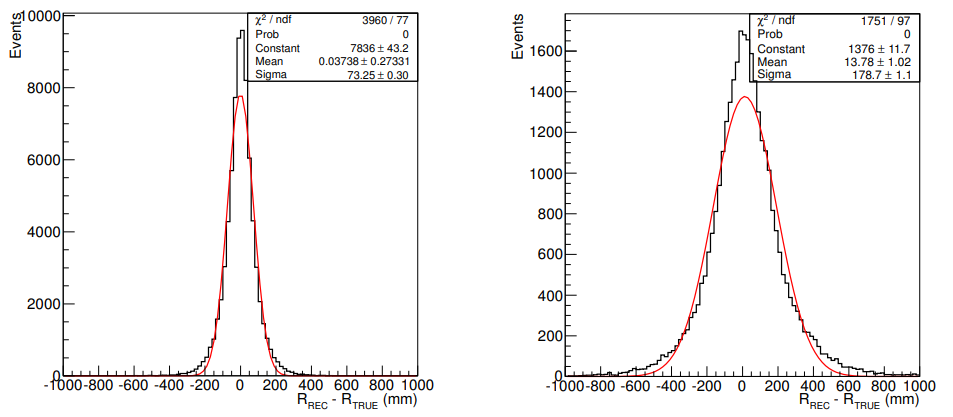
\includegraphics[scale=0.6]{Reconstruction/chargeTemp_bias_r.png}
  \caption{Distributions of residuals of the radial coordinate for the AdSimple charge template vertex reconstruction. IBD positrons are shown on the left, while IBD nGd captures are shown on the right.}
  \label{fig:chargeTemp_bias_r}
\end{figure}

\begin{figure}[h]
  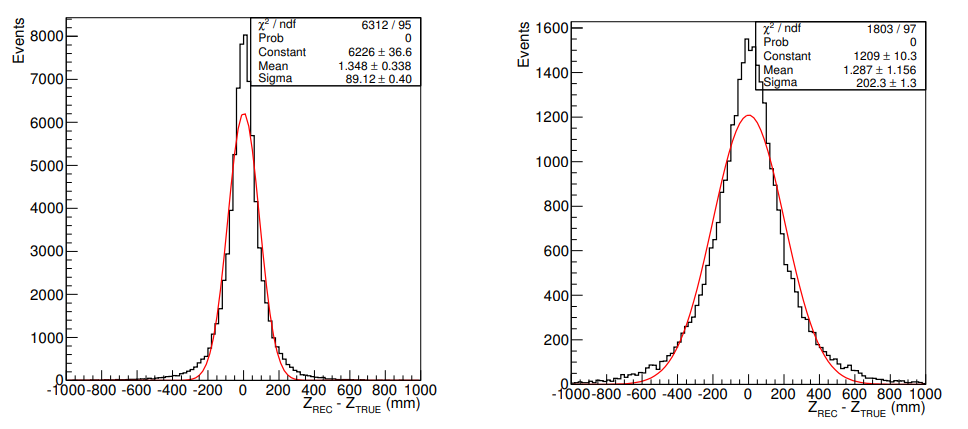
\includegraphics[scale=0.6]{Reconstruction/chargeTemp_bias_z.png}
  \caption{Distributions of residuals of the vertical coordinate for the AdSimple charge template vertex reconstruction. IBD positrons are shown on the left, while IBD nGd captures are shown on the right.}
  \label{fig:chargeTemp_bias_z}
\end{figure}

\begin{figure}[h]
  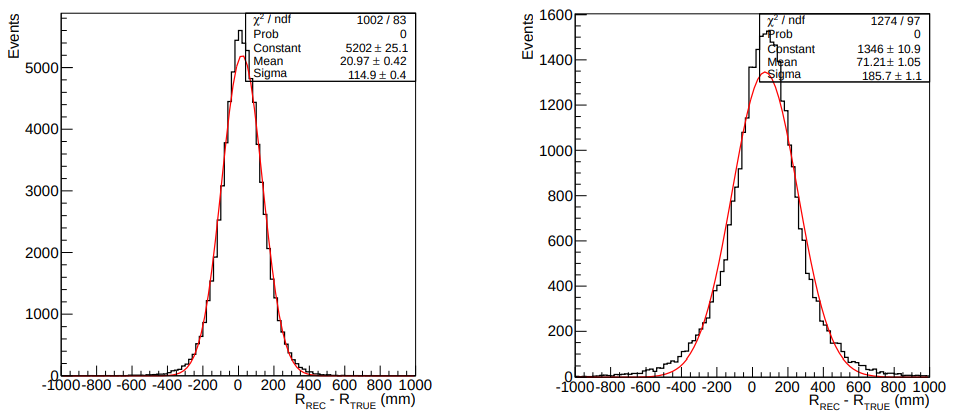
\includegraphics[scale=0.6]{Reconstruction/mccCoc_bias_r.png}
  \caption{Distributions of residuals of the radial coordinate for the AdSimple MC-corrected center of charge vertex. IBD positrons are shown on the left, while IBD nGd captures are shown on the right.}
  \label{fig:mccCoc_bias_r}
\end{figure}

\begin{figure}[h]
  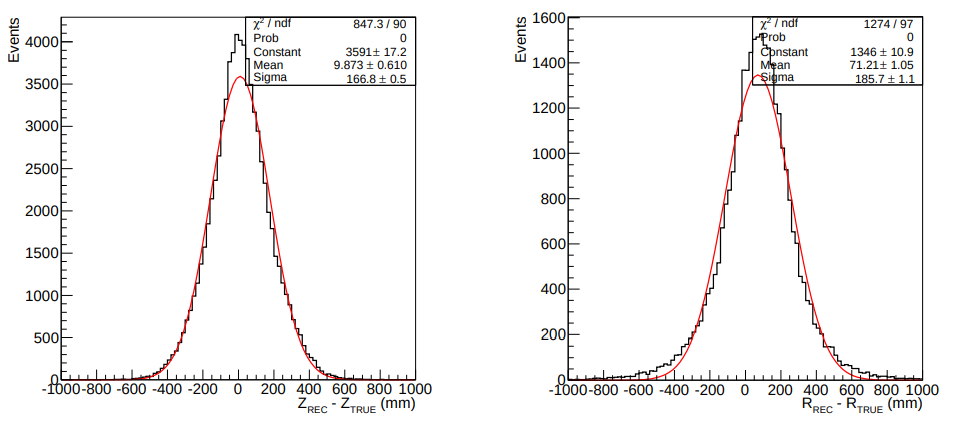
\includegraphics[scale=0.6]{Reconstruction/mccCoc_bias_z.png}
  \caption{Distributions of residuals of the vertical coordinate for the AdSimple MC-corrected center of charge vertex. IBD positrons are shown on the left, while IBD nGd captures are shown on the right.}
  \label{fig:mccCoc_bias_z}
\end{figure}

Note that the reconstructed vertex is not directly used in selecting IBD candidates in this analysis. However, it is still used indirectly in calculating the reconstructed energy (via the nonuniformity correction). In addition, some studies of background rates and spectra also depended on the reconstructed vertex. Finally, there is an independent oscillation analysis (not covered in this thesis), based on selecting IBDs where the neutron is captured on hydrogen, and this one typically relies on the use of the prompt-delayed distance in order to reduce the background of accidental coincidences.

\end{document}